\chapter{Basic principles of RFID}

\section{Contextualization}

The concept of identification with the aid of \ac{rf} dates back to the late 1930s. During the World War II, both fronts were using radar technologies to detect approaching planes. The problem was to identify if planes were allies or enemies.

The German aircraft force, \emph{Luffwaffe}, found out that as pilots rolled their planes, it would change the radio signal reflected back. This system could identify German aircrafts from Allies, being roughly the first \ac{rfid} passive application~\footnote{passive as it didn't need a powered \ac{rf} transmitter in the object to be identified}.~\cite{dobkinRFRFIDPassive2007}

It was soon later, that Watson-Watt, under a British project, developed the first \ac{rfid} active application for \ac{iff} system. An active \ac{rf} transmitter was attached to British planes, which on receiving radar signals from base stations, broadcasted a signal identifying the aircraft has allied.~\cite{HistoryRFIDTechnology}

This established the core concept of today's systems that make this dissertation possible - the over the air identification of transponders~\footnote{a device that, upon receiving a signal, emits a different signal in response}.

The technology kept advancing through the 1950s and 1960s, mainly in the academic field. Companies started to commercialize anti-theft systems based on 1-bit tag~\footnote{a simple inductive RC resonant circuit that detects transponders in field by changes in the reader coil voltage~\cite{andreventuradacruzmarnotozuqueteIdentificacaoPorRFID2018}}.

In the 1970s the first patents were registered on active tag with rewritable memory and a passive transponder for door lockers. The \ac{us} National Laboratory of Los Alamos was asked, by the Energy Department, to developed a tracking system for nuclear materials. The Agricultural Department also requested Los Alamos for a animal tracking system that was design based on \ac{uhfrfid}. These technologies were also transposed by the same engineers to automated toll payment systems in the private market~\cite{landtHistoryRFID2005, HistoryRFIDTechnology,casierAnalogCircuitDesign2011}.

The 1980s experienced the boom of \ac{rfid} development with wager by the private industries and the development of the personal computer.

The 1990s, with the growing and high deployment of the technology, the first standards were developed. 

The 2000s followed the same maturation process but with slow adoption rate in the late part of the decade. 
Despite the interest presented by the retail giants, like Wal-Mart, and investment by the \ac{dod}, the compromises created by the \ac{rfid} industry didn't justified the commitment. The high cost for investment, technical performance difficulties, conflicting standards, security issues and privacy concerns made the investment stale~\cite{RFIDAdoptionStalls}. 
Companies had to strangle \ac{rnd} resources due to inexistent tools and complex implementations, which were required to develop tools for the marketing/sales departments, that truly make use of the \ac{rfid} infrastructure to increase revenue.
Making suppliers adapt to \ac{rfid} also seemed to be a problem, since many companies don't have \ac{rnd} resources at all to begin with~\cite{gaudinSuppliersGainFailed2008}.
Another big issue was the standardization of coding schemes in RF tags. The fight for dominance in the \ac{uhfrfid} market led to multiple coding standards and protocols that made inter-operation among vendor and suppliers infeasible, if not impossible.

In the last decade, despite the advancements in the industry and the adoption by big apparel retailers like Zara, Decathlon and Marks \& Spencer~\cite{RFIDRetailApparel}, there are issues that could inhibit wide-scale use which will be discussed in section~\ref{currentproblems}.

\section{RFID System}

\ac{rfid} is an automatic identification technology that uses radio waves or magnetic fields to identify physical objects.

\emph{Automatic identification} technology refers to technology that automatically identify objects and collects data about them.
Under these technologies we can find the bar code, QR code, biometric (e.g. fingerprint and retina scan), voice identification, \ac{ocr} and the focus of this dissertation, \acl{rfid}. 

In fact, currently, \ac{rfid} is more than just an \emph{identification} technology. Tags have a good amount of storage which can be used to keep information about all kinds of business information, e.g. expiration date, batch number, technical and maintenance information, etc.

An \ac{rfid} system is a collection of components that implement an \ac{rfid} solution. In the most simplified demonstration, an \ac{rfid} system starts with a radio device called tag~\footnote{the technical term is transponder, but the common term and most used transponder is a tag, which will be used through out the thesis instead}. The tag is attached to the object that needs to be identified. When such a object is presented in front of an antenna connected to a suitable \ac{rfid} reader, the tag transmits this data to the reader via the reader antenna. The reader then forward the information through a communication channel to a software application running on a computer. This information then can be used for all kids of applications.

\section{\acl{em} Concepts}

\ac{rfid} technologies use \ac{em} fields or \ac{em} waves to transmit information back and forward between reader and tag.
Designing a well performant system requires a good understanding of \ac{em} concepts.
Reading distance, costs, material properties of tagged object and \ac{rf} environments are a few points where engineers need a good understanding of \ac{em} fields and \ac{em} waves to come up with a good \ac{rfid} solution.

\subsection{\emph{Near-field} and \emph{Far-field}}

An \ac{em} field is the phenomenon produced by moving electric charges. It can be described through Maxwell's equations and mathematical abstracted as a combination of an electric field ($\vec{E}$) and a magnetic field ($\vec{B}$) that interact with each other and their surroundings.
These interactions behavior differently as the distance from the source changes and are usually defined as two main regions: \emph{near-field} and \emph{far-field}.

\subsubsection{\emph{Near-field}}

\emph{Near-field} manifests from the electric and magnetic fields near the charges and current that directly produced them. It is the region where phenomena like \ac{em} induction and electrostatic occur.

This field can be further split in two regions: reactive \emph{near-field} and radiative \emph{near-field}.

Is in the reactive region that \emph{near-field} \ac{rfid} technologies are defined for. It is the closest to the transmitting antenna and is characterized by non-radiative behaviors. In this region, if the energy is not absorbed by a receiver, self-capacitance and self-inductive effects cause the antenna to store energy very near its surface. When electrons from a nearby conductor are placed in this region, field reactive \emph{near-field} energy is transferred to them, resulting in an energy drain on the transmitter by a change in the impedance viewed by the reader.

In the radiative \emph{near-field}, i.e.\ Fresnel region, the back-coupling of the fields becomes out of phase with the antenna signal, and thus cannot efficiently return inductive or capacitive energy from antenna currents or charges.
In this region conductive objects, such as shelve metal structures, can behave as antennas by inductively receiving and then "re-radiating" some of the energy~\cite{ElectromagneticRadiationField}.

In the context of \ac{rfid} technologies, only the reactive zone is considered when referring to the \emph{near-field} region. The radiative zone is \textit{ineffective} and rather unpredictable and usually not accounted referring to \ac{rfid}.

\subsubsection{\emph{Far-field}}

The \emph{far-field} region is the area where the field behaviors as a \textit{normal} radiating field, composed of \ac{em} waves that propagate outwards - i.e.\ electromagnetic radiation.

\ac{em} waves are created as result of uniform vibrations between an electric field and a magnetic field. In other words, \ac{em} waves are composed of oscillating magnetic and electric fields. A change in one of the field components reflects an equal change of the other and one can not exist independently.
These waves are detached from any feedback from the moving charges that produced it. Means that, after the waves leave the transmitter, they are completely independent of both transmitter and receiver, as opposed to the phenomena in the \emph{near-field} region.

In this region the radiated power decreases $1/d^2$ as the distance ($d$) from the reader antenna increases, being the best option for \ac{rfid} technologies requiring high reading distances (e.g.\ \ac{uhfrfid}).

\subsubsection{Boundaries}

The boundaries between these regions are characterized by locations where the activity of the associated field components are the strongest. They can be roughly defined by a few rules of thumb.

Boundaries between fields are roughly delimited by approximately one full wavelength of the \ac{rf} wave emitted from a reader antenna.
This can be more precisely defined taking in account the transmitting antenna characteristics.

For antennas whose size is comparable to wavelength or bigger (used in \ac{uhfrfid}), the \emph{far-fields} boundary can be delimited by the Fraunhofer distance, radial from the antenna. The Fraunhofer distance is described by equation~\ref{eq:fraunhofer}, where $D$ is the largest dimension of the radiator and $\lambda$ the wavelength~\cite{balanisAntennaTheoryAnalysis2005}.

\begin{equation} \label{eq:fraunhofer}
    d_F = \frac{2D^2}{\lambda}
\end{equation}

\begin{figure}[!ht]
    \centering
    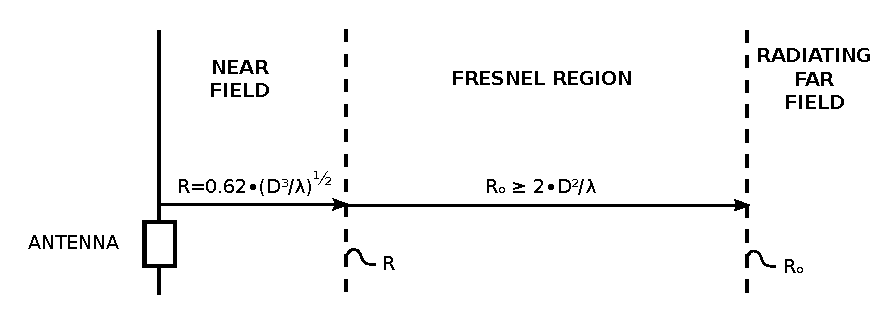
\includegraphics[width=0.9\textwidth]{./figs/02-state-of-the-art/FarNearFields-USP-4998112.pdf}
    \caption{Field for antennas larger than the wavelength of the radiation it emits~\cite{zerodamageFarFieldsVectorized1991}} 
    \label{fig:fieldregionsbigantenna}
\end{figure}

Small antennas, shorter than half of the wavelength of the emitting radiation, (used in \ac{lf}/\ac{hf} \ac{rfid}), the delimited range between regions is given by $r = \lambda / 2\pi = 0.159\lambda$~\cite{nikitinOverviewFieldUHF2007a}. 

\begin{figure}[!ht]
    \centering
    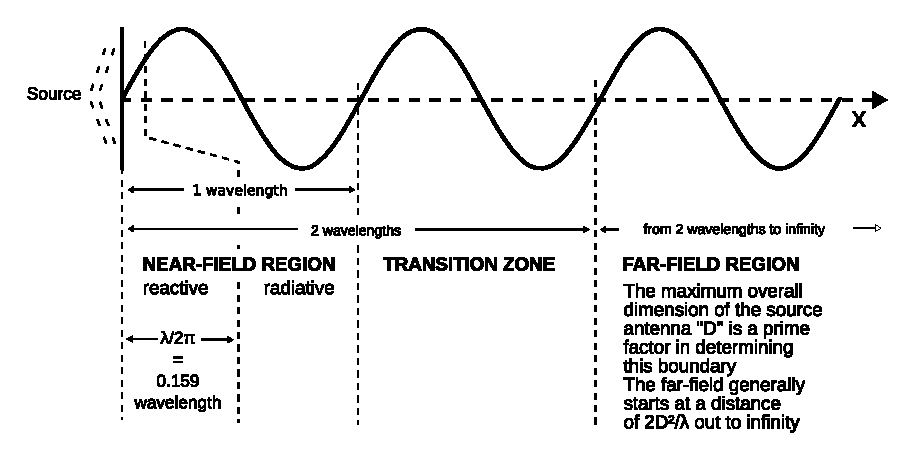
\includegraphics[width=0.9\textwidth]{./figs/02-state-of-the-art/Field_regions_for_typical_antennas_vector.pdf}
    \caption{Fields for antennas equal to, or shorter than, one-half wavelength of the radiation they emit~\cite{SafetyHealthTopics}} 
    \label{fig:fieldregionsshortantenna}
\end{figure}



For \ac{rfid} technologies that depend upon the \emph{near-field}, these ranges are the physical limit between antenna and transponder.


\section{Tag}

An \ac{rfid} tag is a transponder composed by a microchip and an attached antenna that can store and transmit data in a contactless manner using radio waves.

% Near-field (Inductive coupling), Far-field (Backscatter coupling)- Read range depends on:
%- transmitter (reader) power
%- energy requirements of the tags (for passive tags)
%- absorption factor of materials to which the tag is attached
%- tag size: the smaller the tag, the smaller the energy capture area, the shorter the read range

\begin{figure}[!ht]
    \centering
    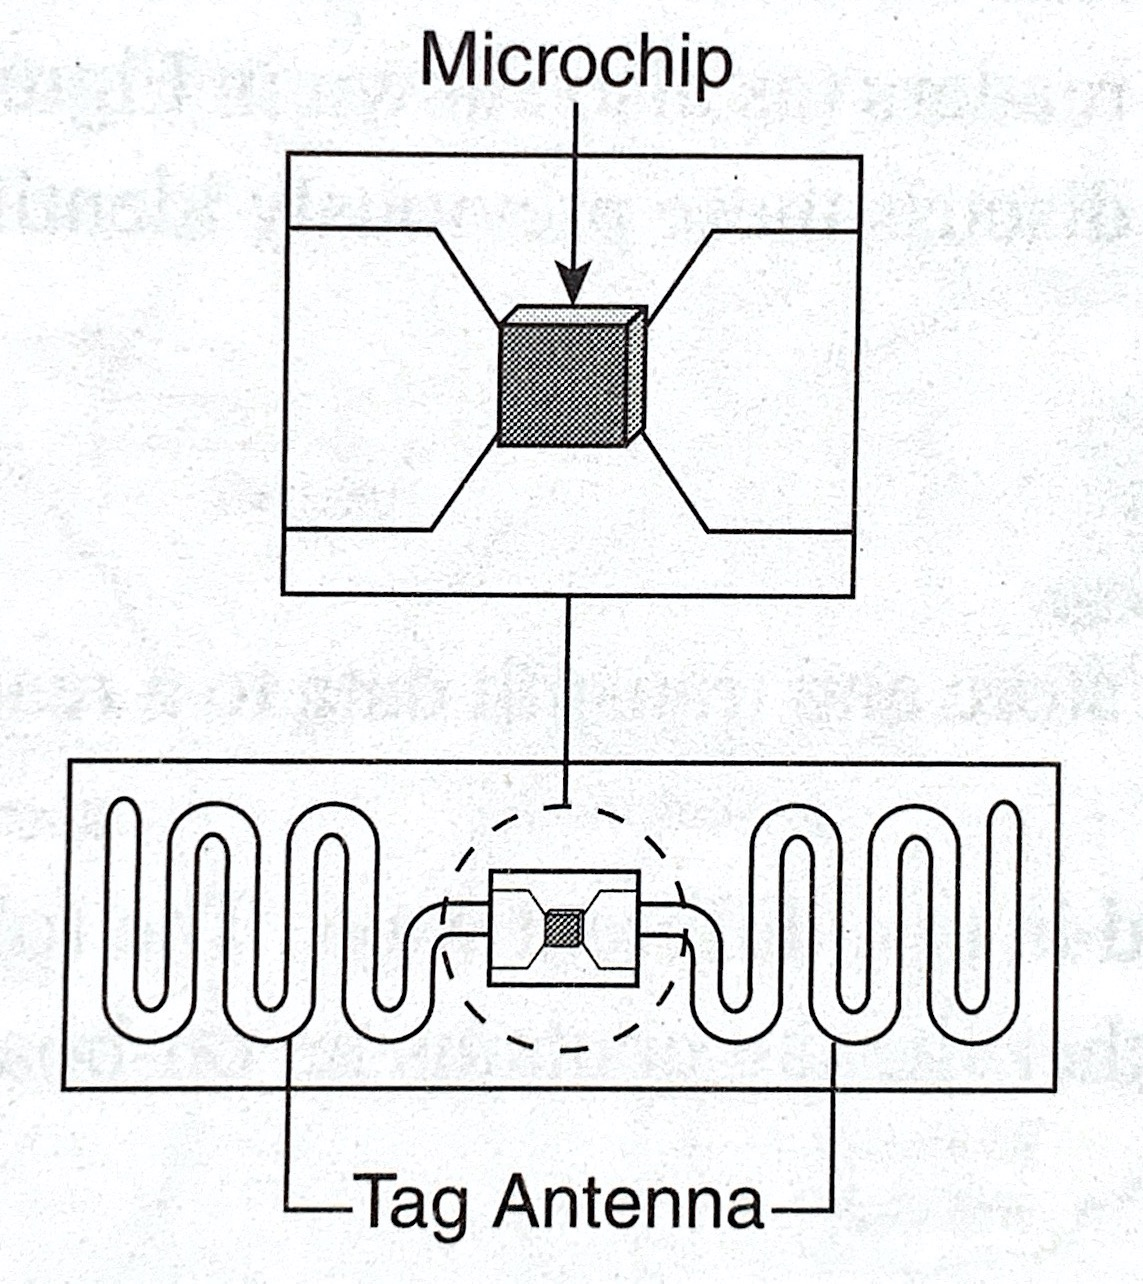
\includegraphics[width=0.2\textwidth]{./figs/02-state-of-the-art/tag.jpg}
    \caption{Components of a passive tag~\cite{lahiriRFIDSourcebook2005}} 
    \label{fig:passivetag}
\end{figure}

%The most common classification characteristics are: power - which is based on whether the tag contains on-board power supply and/or harvest energy from the transmitter \ac{rf} waves; and frequency of operation

%Electromagnetic induction if the production of voltage a conductor situated in a changing magnetic flux

%Faraday found that the voltage produced around closed path conductor is proportional to the rate of change of the magnetic flux through any surface

%A antenna of the reader generates a magnetic fields
%The field induces voltage in the coil of the tag and supplies the tag with energy (Faraday's Law)

%Electromagnetic induction if the production of voltage a conductor situated in a changing magnetic flux

%Faraday found that the voltage produced around closed path conductor is proportional to the rate of change of the magnetic flux through any surface

%\begin{equation}
%    \varepsilon = -\frac{d \Phi_B}{dt}
%\end{equation}

\subsection{Antennas}

% Types: circular, linear .. caracteristics of UHF RFID antenna design 

\section{Technologies}

\ac{rfid} systems are classified by the frequency band they are used in, which differs between applications:

\section{Advantages and Limitations}

% --------------------------------------------------------------------------------------------------------------

%Electromagnetic wave propagation is used for data transmission (and powering transponders in the case of passive tags)

%The reader transmits and electromagnetic (EM) wave which propagates outward

%The amount of energy available is decreasing, $1/d^2$, as the distance from the reader increases

%The receiving or transmitting energy is related to the antenna aperture, which related to the wavelength of the sine-wave

%At this frequencies (UHF) we can control the direction of waves, and thus improve the readability in certain areas \dots



%Antennas can also use different polarization for each wave, and this maximize the transmission of information

%The received power can be related to the transmitted power by using the Friis formula that states:

%\begin{equation}
    %P_T = A_{e2} \frac{P_{in}}{4\pi r^2} G_1 = \frac{\lambda^2}{4\pi} G_2 \frac{P_{in}}{4\pi r^2} G_1 \Leftrightarrow P_T = P_{in}  \bigg(\frac{\lambda}{4\pi r} \bigg)^2 G_t G_r
%\end{equation}